\chapter{Method}

\section{Wavelength Calibration}

Wavelength calibration of the spectrometer was done using three lasers whose wavelengths were first measured with a Burleigh Wavemeter:  a red diode laser at 656.99~nm, a doubled Nd:YAG laser at 532.23~nm, and the C480 blue dye laser typically around 475~nm.  These lasers were directed at the same position on the sapphire window, and their scatter was imaged along the same path as the Ba fluorescence.  The WinSpec software applies the diffraction grating equation to calibrate each CCD pixel to a wavelength.

\section{Fitting of Spectra}
\label{sec:fitting}

Fitting of fluorescence spectra, with sums of peak-specific fit functions, was used to track peak heights in excitation spectra, annealing cycles, and bleaching.  The center and width parameters of the functions were kept fixed, while the heights were the free fitting parameters.  Center and width parameters for each peak were determined by fitting spectra where that peak is relatively large.  Some fine-tuning was done to match slightly different shapes resulting from different excitation wavelengths.

\subsection{Fitting Spectra with Green Excitation}
\label{subsec:fitgrn}

\begin{figure} %[H]
        \centering
                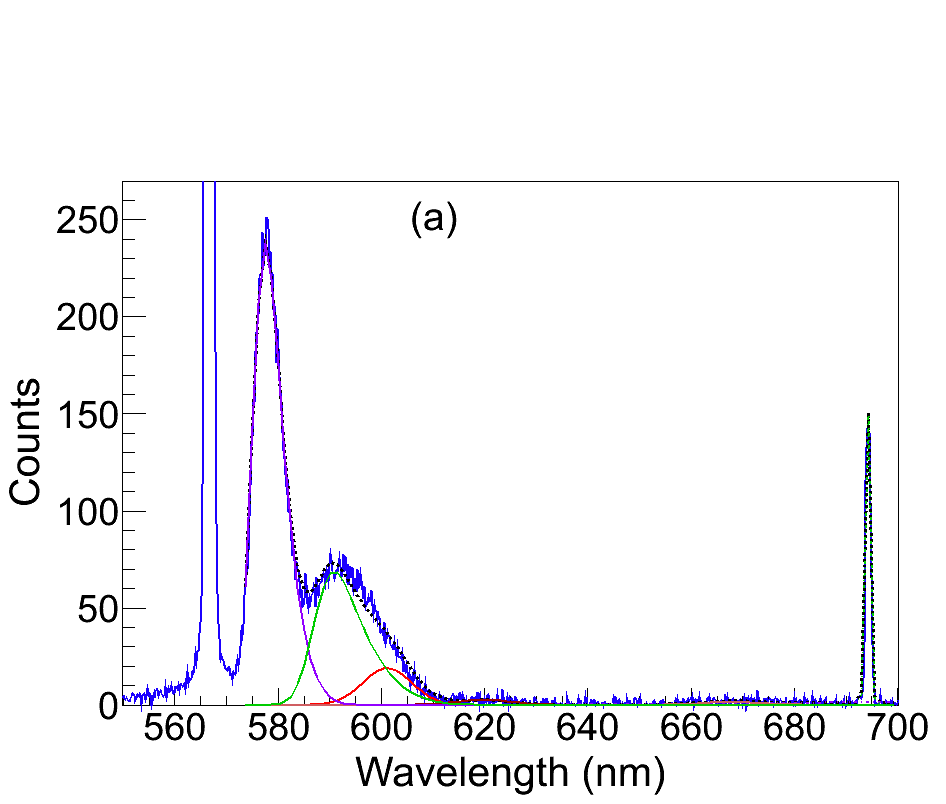
\includegraphics[width=.5\textwidth]{figures/spectra_fit_a.png}
                ~
                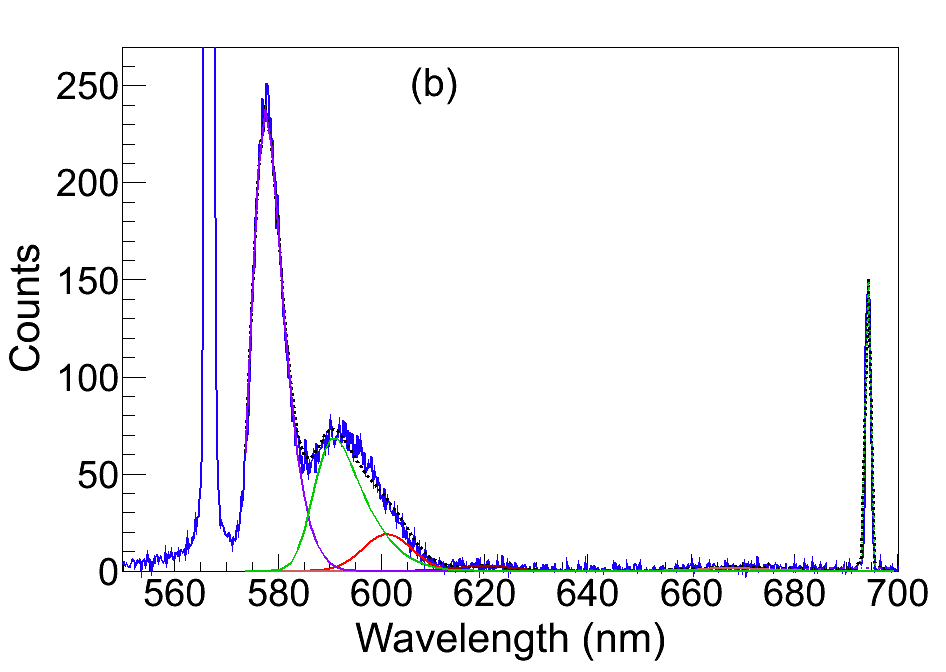
\includegraphics[width=.5\textwidth]{figures/spectra_fit_b.png}
                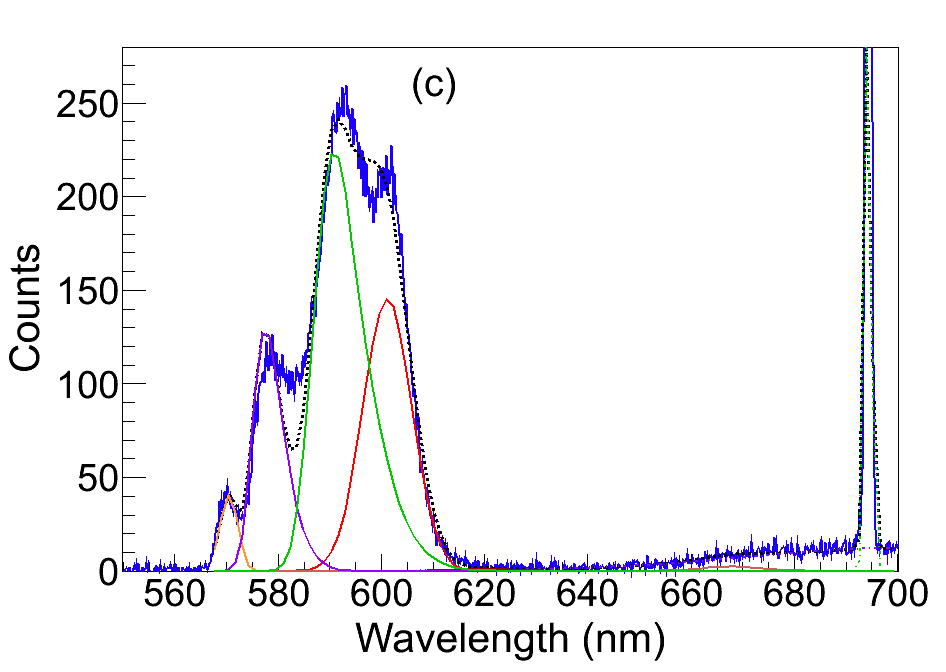
\includegraphics[width=.5\textwidth]{figures/spectra_fit_c.png}
                ~
                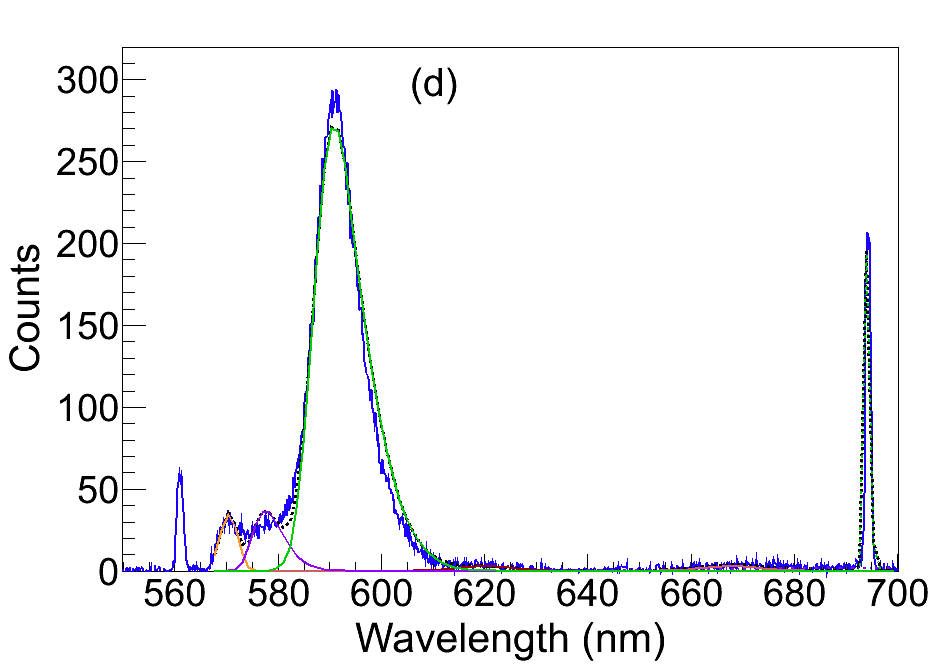
\includegraphics[width=.5\textwidth]{figures/spectra_fit_d.png}
                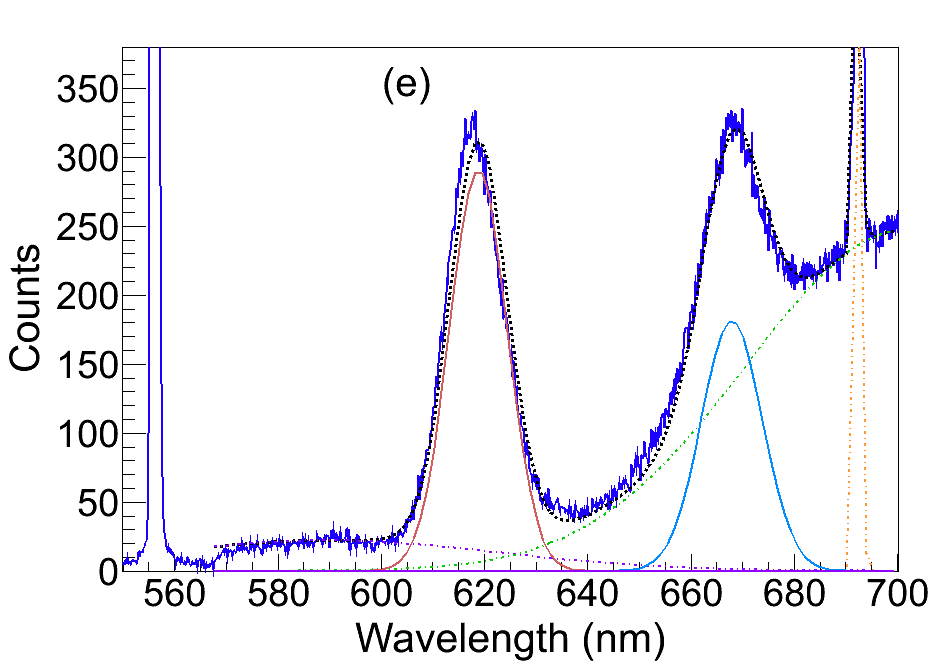
\includegraphics[width=.5\textwidth]{figures/spectra_fit_e.png}
                ~
                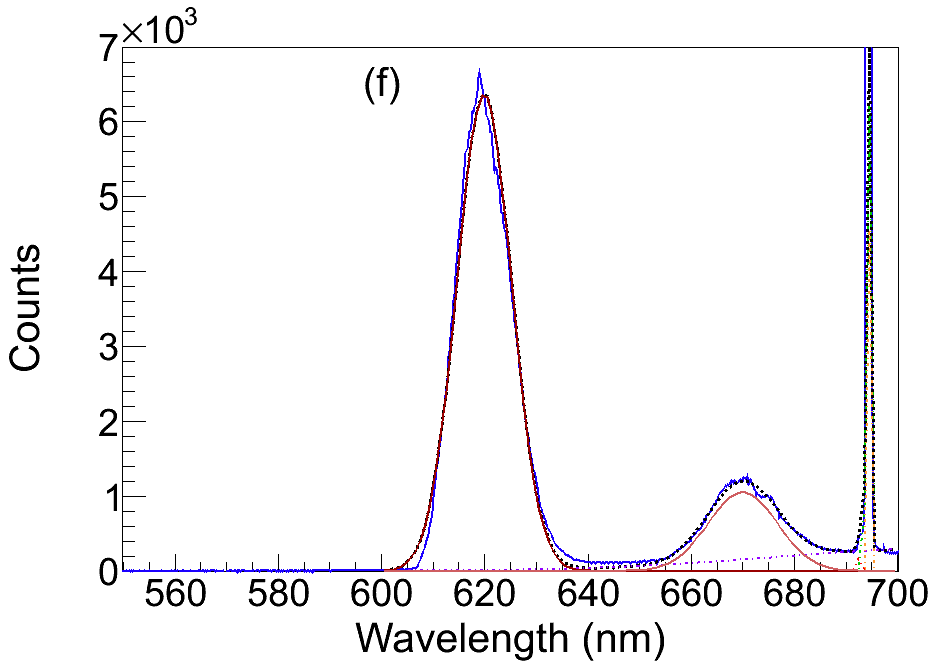
\includegraphics[width=.5\textwidth]{figures/spectra_fit_f.png}
                \caption{Example fits to spectra of Ba\textsuperscript{+} deposits with green excitation at (a) 566.6~nm, (b) 563.4~nm, (c) 546.3~nm, (d) 561.0~nm, (e) 555.9~nm, and (f) 567.3~nm.  Laser scatter can be seen in the lower wavelengths for some figures, especially in (a) where it is on the edge of the Raman filter cutoff.}
\label{fig:specFitsGrn}
\end{figure}

Example fits to spectra of Ba\textsuperscript{+} deposits for several different green excitation wavelengths are shown in Fig. \ref{fig:specFitsGrn}.  To incorporate the tail in the shape of the 577- and 591-nm peaks, an asymmetric function of the form $A(1+$erf$(\frac{x-a}{\sigma_{1}})(1-$erf$(\frac{x-a}{\sigma_{2}}))$ was used, where $a$ is the fixed center-defining parameter, $\sigma_{1}$ and $\sigma_{2}$ are fixed left and right width parameters, and $A$ is the free amplitude parameter.  The function erf() is an error function.  The 570-, 601-, 619-, and 670-nm peaks were fit with Gaussian functions with fixed widths ($\sigma$) of 1.7~nm, 4.7~nm, 5.3~nm, and 6.7~nm, respectively.  Rather than attempting frame-by-frame background subtractions, additional Gaussians were fit to the broad and sharp background fluorescence.  Two broad Gaussians centered at around 590~nm and 702~nm, and one sharp Gaussian at 694~nm, were chosen by fitting spectra of Xe-only deposits.  These backgrounds and their excitation spectra are discussed in \ref{sec:bgs}.  The full fit, i.e. the sum of each contributing peak fit, is the dotted black line.  Though the shapes do not match perfectly for all excitation wavelengths, the fits still follow the peak amplitudes well.  Ba emission and excitation spectra results are discussed in Sec. \ref{sec:fluorescence}.

\subsection{Fitting Spectra with Blue Excitation}
\label{subsec:fitblu}

Example fits to spectra of Ba\textsuperscript{+} deposits for several different blue excitation wavelengths are shown in Fig. \ref{fig:specFitsBlu}.  Gaussian functions were used for 532-, 568-, and 575-nm peaks with widths ($\sigma$) of 2.4~nm, 5.0~nm, and 0.7~nm, respectively.  Lorentzian functions were used for the 553-, 592-, 635-, and 669-nm peaks with widths ($\gamma$) of 1.7~nm, 13.8~nm, 10.4~nm. and 9.1~nm, respectively.  Similar to spectra with green excitation, the background components were fit with two broad Gaussians centered at 546.0~nm and 703.3~nm, with respective $\sigma$ of 49.0~nm and 30.5~nm, as well as one sharp Gaussian centered at 693.4~nm peak with $\sigma$ of 0.5~nm.  The fits around 478~nm (e.g., (c)) are not quite right, mainly due to a shift in central value of the 592-nm peak.  However, fit values still follow respective peaks heights well.  The 522- and 575-nm peaks are seen in (c), though the 522-nm peak is left out of the fitting range since it sits on the Raman filter cutoff.   These spectra are discussed in Sec. \ref{sec:BaPlus}.

\begin{figure} %[H]
        \centering
                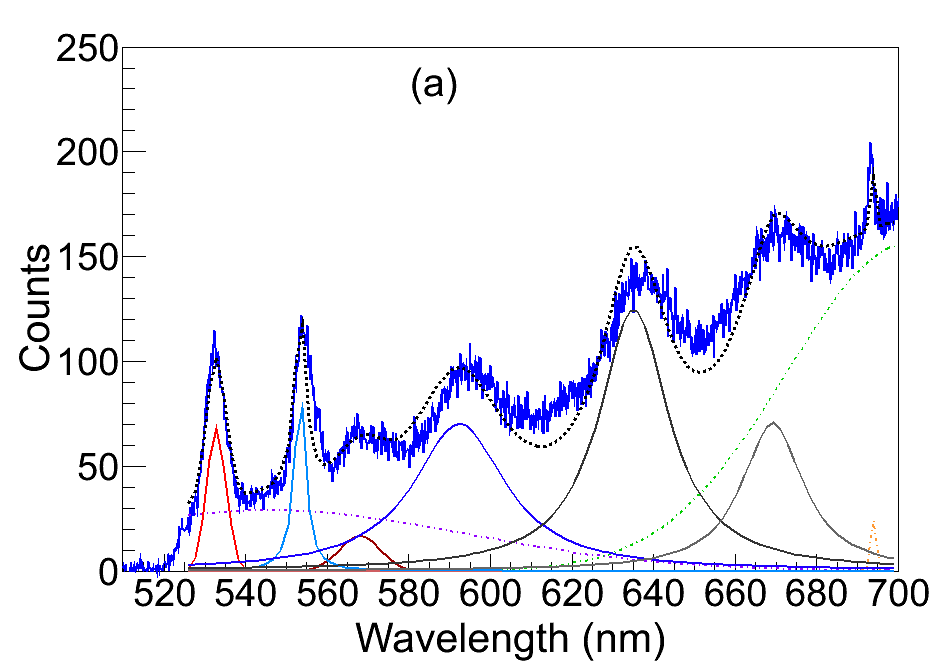
\includegraphics[width=.5\textwidth]{figures/spectra_blu_fit_a.png}
                ~
                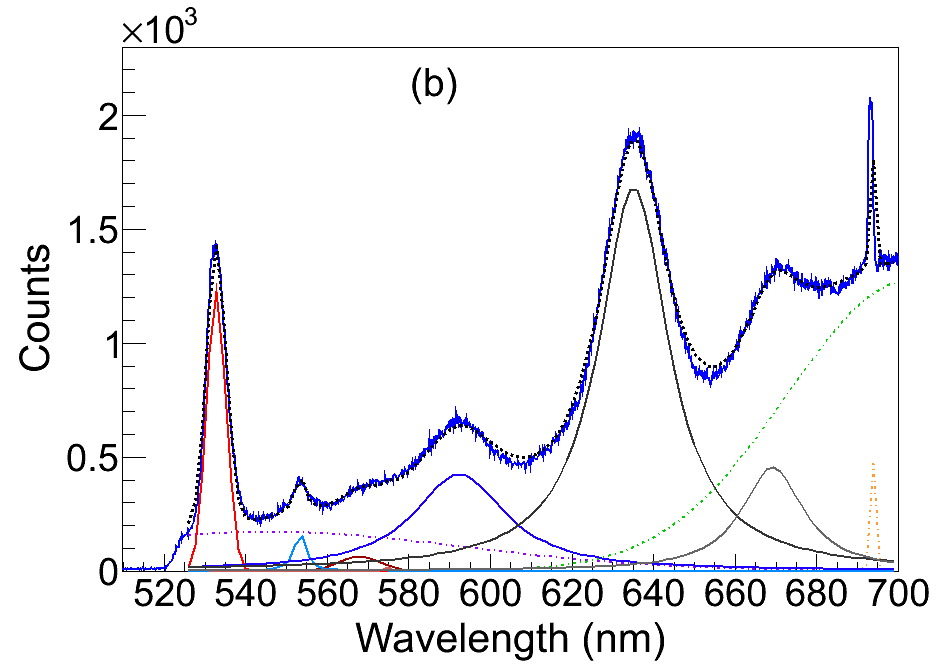
\includegraphics[width=.5\textwidth]{figures/spectra_blu_fit_b.png}
                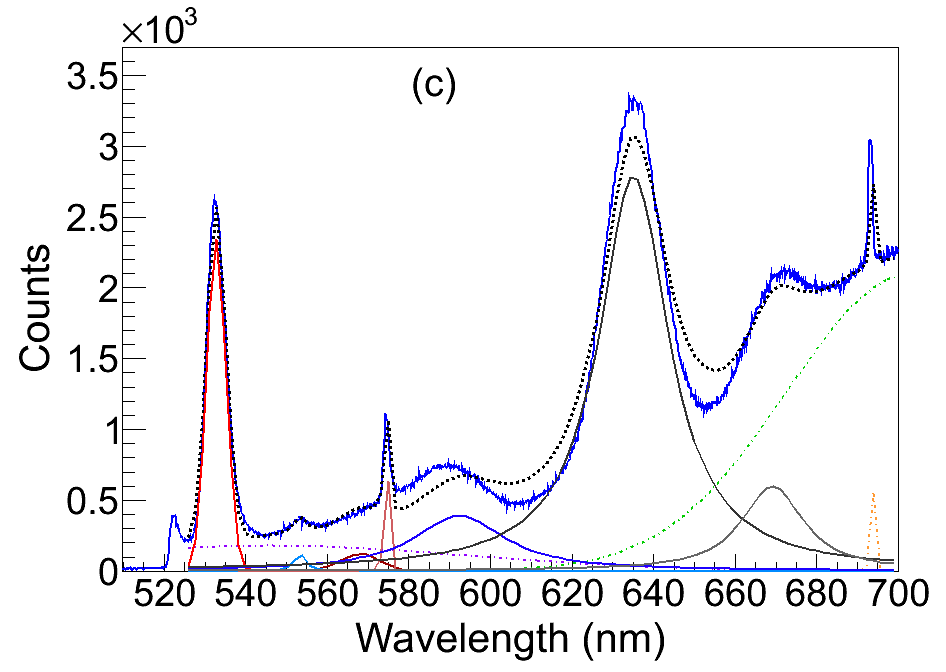
\includegraphics[width=.5\textwidth]{figures/spectra_blu_fit_c.png}
                ~
                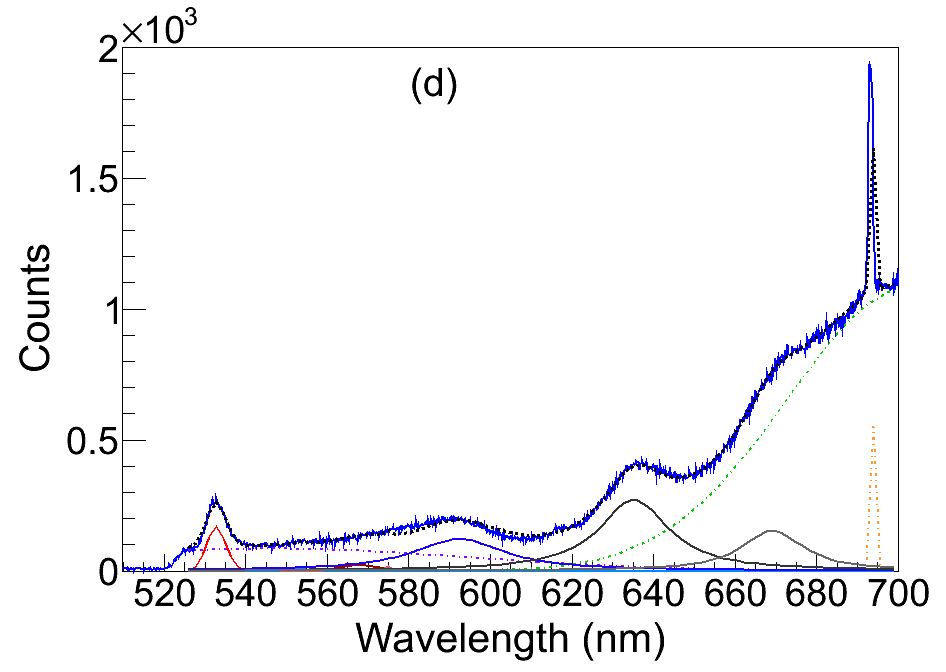
\includegraphics[width=.5\textwidth]{figures/spectra_blu_fit_d.png}
                \caption{Example fits to spectra of Ba\textsuperscript{+} deposits with blue excitation at (a) 461.7~nm, (b) 468.2~nm, (c) 478.3~nm, and (d) 488.2~nm.}
\label{fig:specFitsBlu}
\end{figure}

%\emph{results section, moved here: The broad blue BG ... what does its excitspec look like? is it possible it is the surface BG? ... anyway you need to mention it.  You need to figure what happened to the BG strangeness.}

%another sprectrum showing partial 601 nm is 20141107 run95.91 (547.0 nm excit.)

%i think you can leave this out: Curves in (a) have about 100$\times$ the laser power used in the excitation spectrum (e.g. (b)) where low intensity is desired to avoid bleaching during the scan.  

%A 566~nm Raman filter was used to attenuate the majority of the laser scatter, however the small amount of scatter passed by the filter was used to determine the frame's excitation wavelength.  Each peak's fit contribution was then integrated and scaled by the frame's laser power, as the power output is not constant through the dye range.

\section{Optimizing Signal-to-Background}
\label{sec:bgs}

One source of background emission was observed from the surfaces of the window.  Its broad fluorescence is shown in Fig. \ref{fig:surfBG}(a) with a 610-nm Raman filter cutoff and 570.4~nm excitation, and its excitation spectrum is shown in Fig. \ref{fig:surfBG}(b) over the R6G dye range.  The nature of this emission has not been determined, however a few features were identified.  One was that the emission increased as the window temperature was decreased, down to about 100~K where it remained flat down to 11~K, shown in Fig. \ref{fig:BGtempDependence}.  Another feature of the surface background is that it bleaches with laser exposure.  In order to reduce this background in imaging experiments, as well as to reduce run-to-run variation in the background due to bleaching, the sapphire window was pre-bleached for at least half an hour.  Decay of the surface background emission, with intermittent observation during a pre-bleaching process, is shown in Fig. \ref{fig:surfBGbleach}.  For efficient pre-bleaching, the dye laser tuned to 580.5~nm for higher laser power, though the observation points in Fig. \ref{fig:surfBGbleach} are taken with the dye laser at 570~nm with the same laser power used in the following Ba imaging experiment.  During imaging experiments, frequent Xe-only deposits were made in order to track surface background emission to establish proper background subtraction.

\begin{figure} %[H]
        \centering
                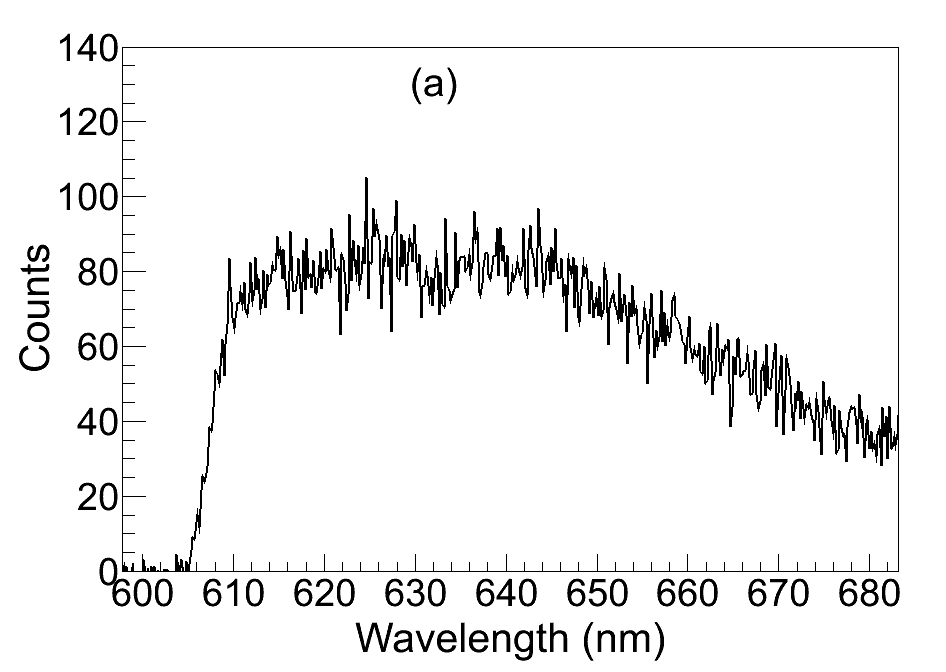
\includegraphics[width=.5\textwidth]{figures/surfaceBG_a.png}
                ~
                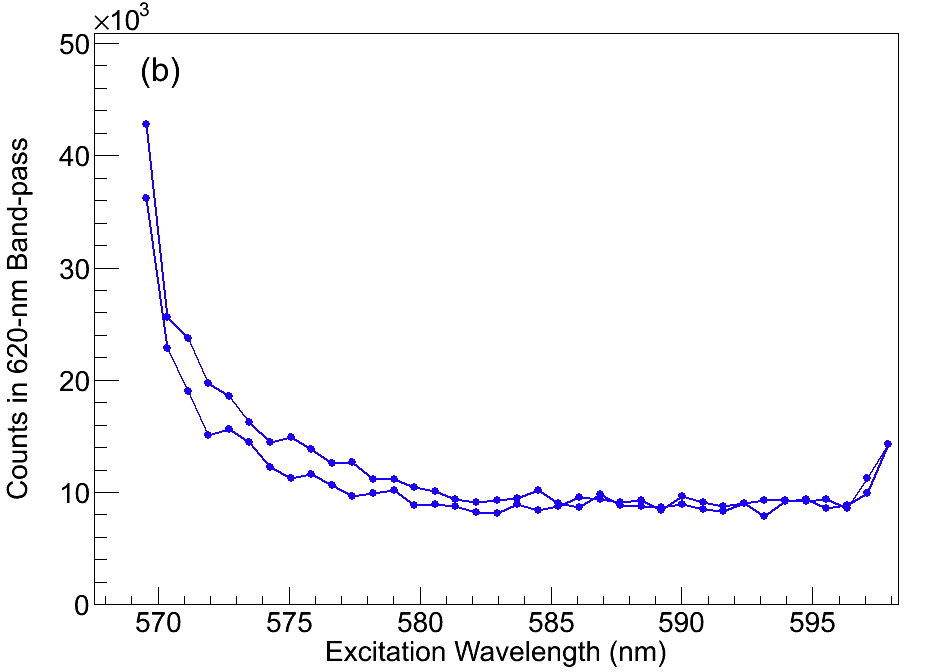
\includegraphics[width=.5\textwidth]{figures/surfaceBG_b.png}
                \caption{(a) Surface background emission spectrum w/ excitation at 570.5~nm, and (b) excitation spectrum through wavelengths in R6G dye range.  The sharp drop in (a) around 608~nm is the Raman filter cutoff.}
\label{fig:surfBG}
\end{figure}

%\begin{figure} %[H]
%        \centering
%                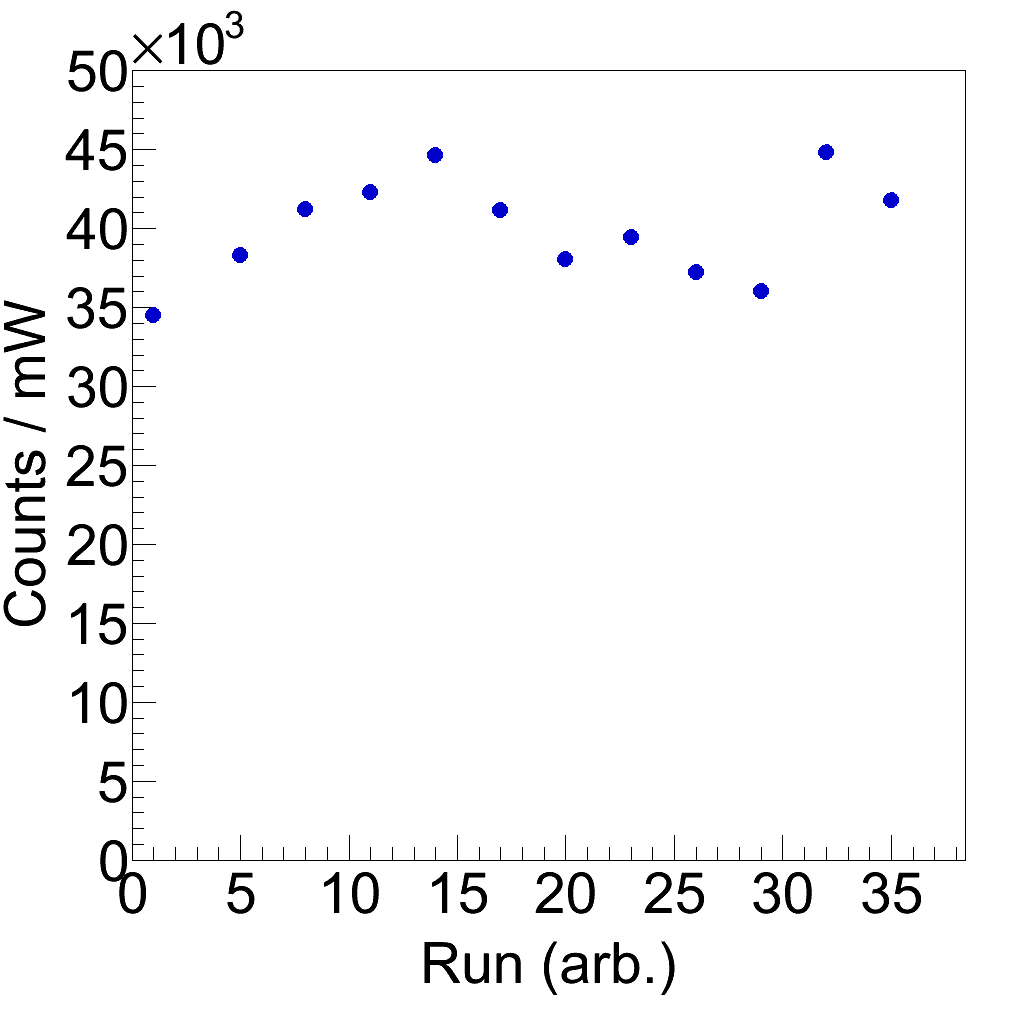
\includegraphics[width=.4\textwidth]{figures/xe_variation.png}
%                \caption{Background counts in focused laser region over the course of an experiment.}
%\label{fig:xevar}
%\end{figure}

%\emph{\color{gray}from results} Variation in the background level, dominated by the surface background, is shown in Fig. \ref{fig:xevar}.  Variation was most likely caused by drift of the laser position on the window, to regions of different historical bleaching.  Local variations are at the single-atom signal level, however positive signal after subtraction, even at the single-atom level, demonstrates that this variation is sufficiently low.

%Spacial variation in the background is especially cumbersome in a laser scanning experiment, as discussed in \ref{sec:scanning}. 

%speculation:    Given these behaviors, it is possible that the surface background is caused by a species which freezes to the window, or something which coats the window and fluoresces more at lower temperatures.  In either case, the bleaching could be explained by evaporation with laser heating, or by optical pumping of the species into a metastable state.

\begin{figure} %[H]
        \centering
                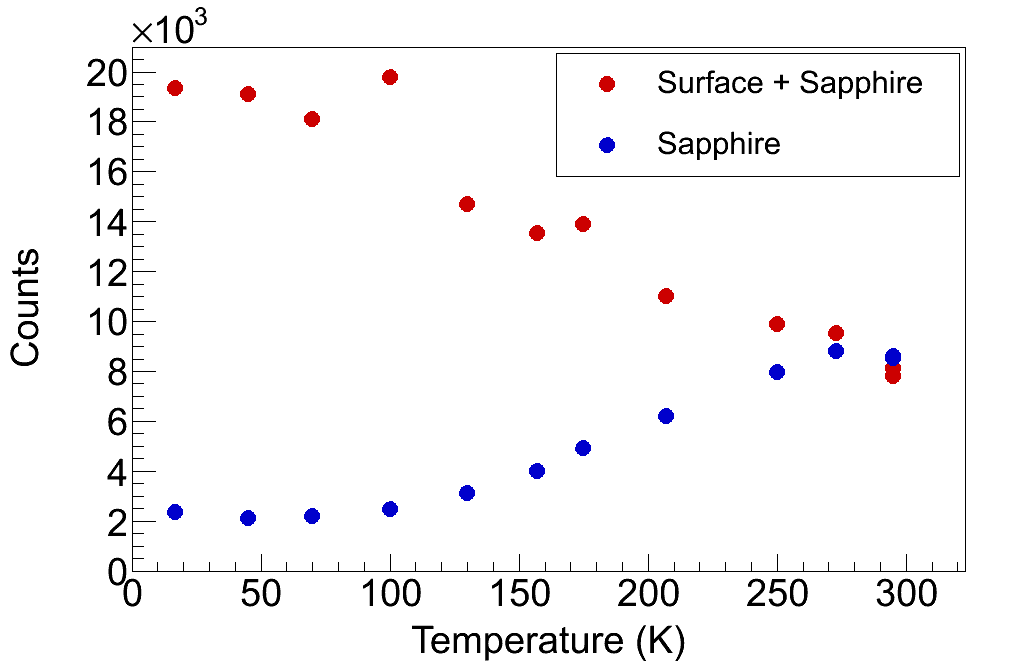
\includegraphics[width=.6\textwidth]{figures/bg_temp_dep.png}
                \caption{Temperature dependence of surface (red) and sapphire bulk (b) backgrounds.}
\label{fig:BGtempDependence}
\end{figure}

\begin{figure} %[H]
        \centering
                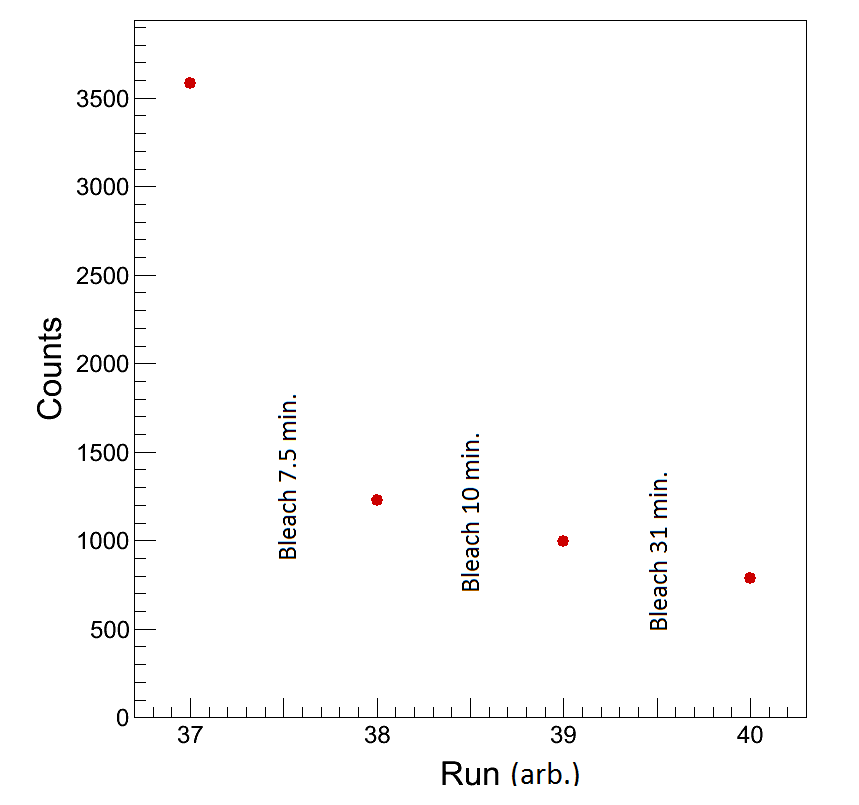
\includegraphics[width=.4\textwidth]{figures/Bleach_SurfaceBG_20150807_part1.png}
                \caption{Decay of surface background emission during pre-bleaching of the sapphire window.}
\label{fig:surfBGbleach}
\end{figure}

\begin{figure} %[H]
        \centering
                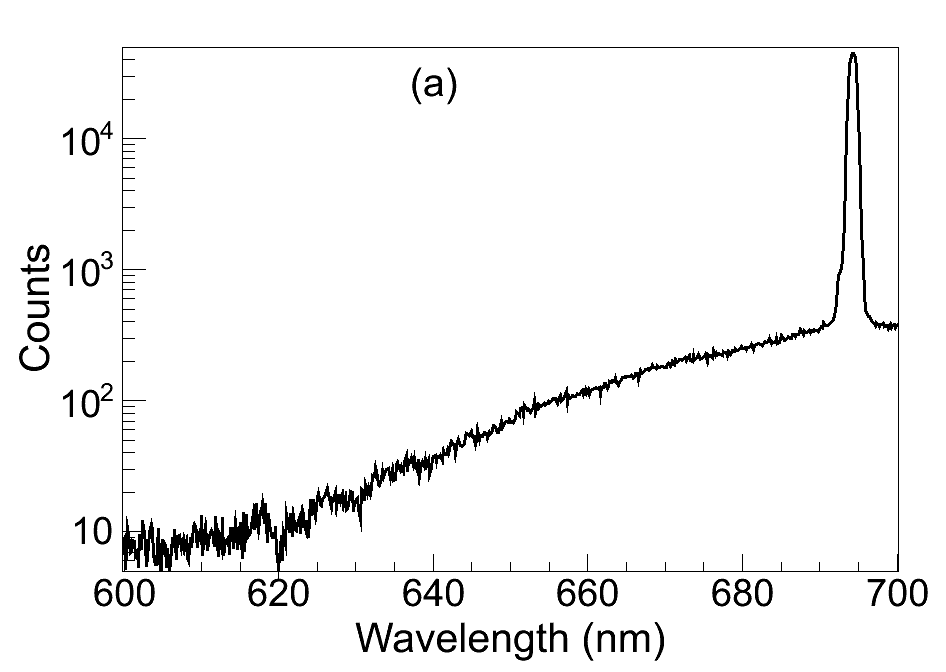
\includegraphics[width=.5\textwidth]{figures/Cr_a.png}
                ~
                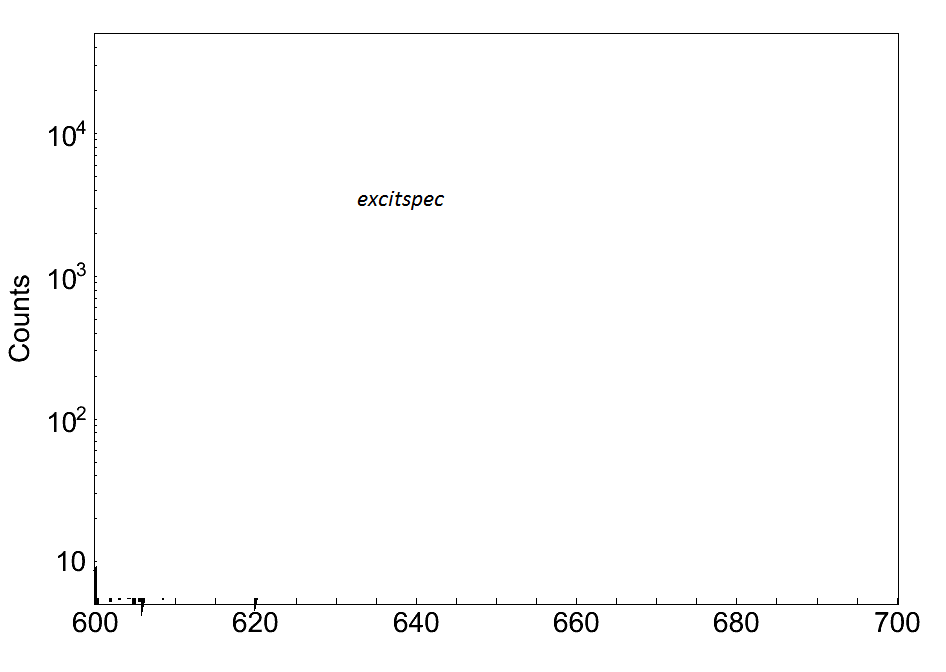
\includegraphics[width=.5\textwidth]{figures/Cr_b.png}
                \caption{(a) Sapphire bulk emission with 562-nm excitation at 11~K, and (b) excitation spectrum of the sharp 694-nm emission peak using three different laser dyes.  Due to different laser powers and exposure times, the R110 and R6G were scaled to match at their boundary.}
\label{fig:Cr}
\end{figure}

\begin{figure} %[H]
        \centering
                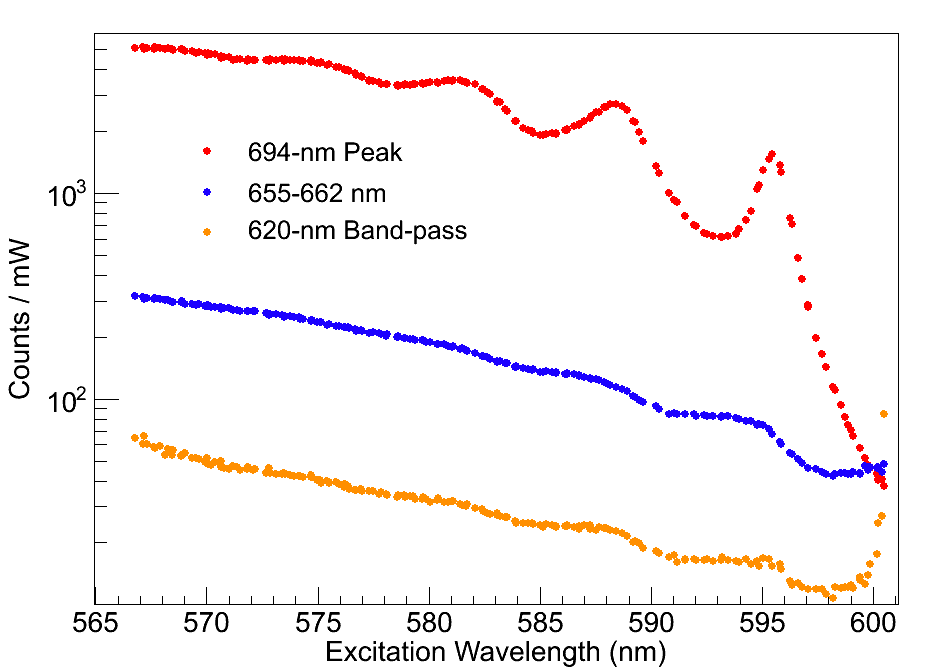
\includegraphics[width=.7\textwidth]{figures/Cr_broad.png}
                \caption{Excitation spectra for weaker sapphire bulk emissions (blue,orange) along with that of the strong 694-nm emission (red).}
        \label{fig:CrBroad}
\end{figure}

Another source of background is fluorescence from the sapphire window bulk.  A spectrum of this fluorescence with 562~nm excitation is shown in Fig. \ref{fig:Cr}(a).  The strong, sharp peak at 694~nm is a well-known $^{2}E$ - $^{4}A_{2}$ emission in the $d^{3}$ configuration of Cr\textsuperscript{3+} impurities in the sapphire bulk \cite{SapphireRlines1964,SapphireRlines2010}.  An excitation spectrum for this peak is shown in Fig. \ref{fig:Cr}(b) over the range all three dyes R6G, R110, and C480, using a sapphire window with relatively high Cr\textsuperscript{3+} content.  Multiple features observed in the excitation spectrum, obtained by integrating the 694-nm peak fit (Sec. \ref{sec:fitting}) vs. excitation wavelength, are consistent with the absorption spectrum of Cr\textsuperscript{3+} in sapphire at 77~K, including three sharp peaks in the blue at 468.4, 474.8, and 476.5~nm, as well as a broad absorption in the green/yellow, peaking around 550~nm, with vibrational peaks on the red tail \cite{SapphireFord,SapphireMcclure}.  In addition to the 694-nm peak, a weaker and much broader emission is observed, along with three weak peaks around the 619-nm Ba peak region, also from the sapphire bulk.  Excitation spectra for these fluorescence components are shown in Fig. \ref{fig:CrBroad} for the R6G dye range.  In this experiment, the laser was de-focused to about w = 200~$\mu$m, and the emission observed was had contribution of the surface background as well as the bulk sapphire emission.  This is negligible for the prominent 694-nm peak, however the rising features of the surface background emission, near 600~nm and 567~nm, can be seen in the excitation spectra of the weaker components (blue, and especially orange curves in Fig. \ref{fig:CrBroad}).  Nonetheless, observation of the same vibrational peaks as in the 694-nm peak demonstrates that the broad emission and weak peaks in the 620 band-pass (Fig. \ref{fig:Cr}(a)) are also due to Cr\textsuperscript{3+} in the sapphire.  Commercially available c-plane quality sapphire windows contain low concentrations of Cr\textsuperscript{3+}.  Sample windows of 0.75" diameter and 0.02" thickness from a few companies were tested, and those from Meller Optics produced the lowest sapphire bulk emission in the 620-nm band-pass region.

\begin{figure} %[H]
        \centering
                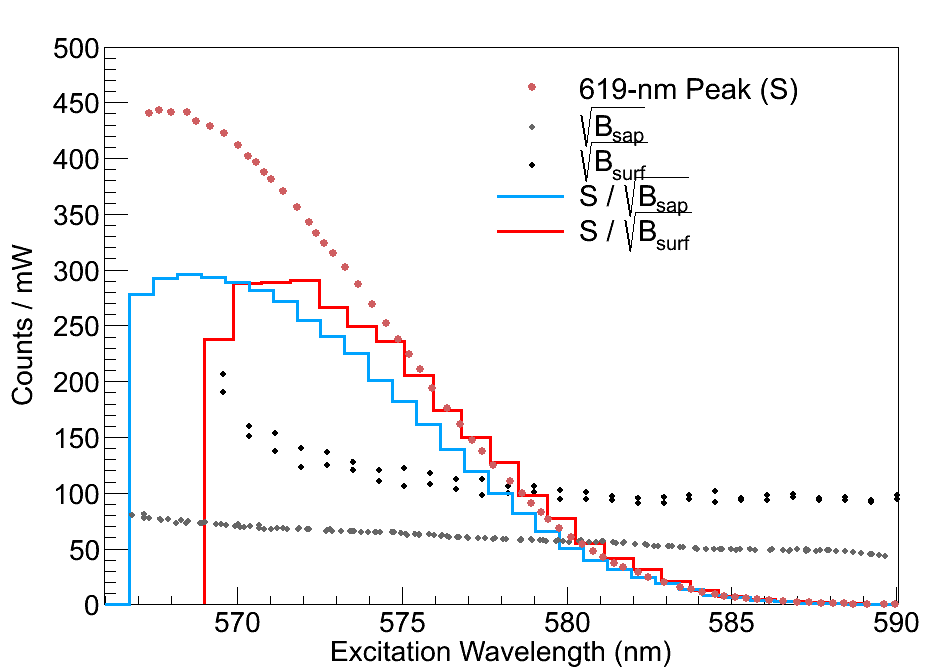
\includegraphics[width=.7\textwidth]{figures/S_to_B_both.png}
                \caption{Optimization of signal to background with the 619-nm fluorescence signal (S) for emission from the surface background (B$_{\text{surf}}$, red) and for the bulk sapphire emission (B$_{\text{sap}}$, cyan).}
        \label{fig:StoB}
\end{figure}

Consideration of signal-to-background ($S$/$\sqrt{B}$) guided the choice of 570~nm for excitation of the 619-nm fluorescence.  $S$/$\sqrt{B}$ for emission passed by the 620-nm band-pass filter is plotted vs. excitation wavelength in Fig. \ref{fig:StoB} for the surface background (B$_{\text{surf}}$) as well as for the sapphire bulk emission (B$_{\text{sap}}$).  The peak in $S$/$\sqrt{B}$ represents the optimal excitation wavelength respective to each of the two background sources.  Around 568.5~nm is optimal vs. the sapphire emission, and around 571~nm is optimal vs. the surface background emission. 570~nm, which was used in sensitive imaging experiments, is nearly optimal in both cases.

%Consideration of signal-to-background ($S$/$\sqrt{B}$) guided the choice of 570~nm for excitation of the 619-nm fluorescence.  $S$/$\sqrt{B}$ is plotted vs. excitation wavelength in Fig. \ref{fig:StoB} for the surface background (B$_{\text{surf}}$) as well as for combination of the surface background and sapphire bulk emission (B$_{\text{sap + surf}}$).

%The Cr\textsuperscript{3+} emission has an inverse relationship with temperature, shown in Fig. \ref{fig:BGtempDependence}.

%with Cr\textsuperscript{3+} concentrations of around {\color{red}10 ppt} observed.

%(peaks around? May need to ask Bill about what peaks exist and at what temps ... a new idea is to just leave it vague, as ``peaks" since you're sure there are at least 2, but vauge is OK)
